\documentclass[oneside]{jufethesis}
\usepackage{enumerate}
% \usepackage{indentfirst}
% \usepackage{setspace}
% \usepackage{geometry}
% \geometry{left=85.05pt,right=85.05pt,top=85.05pt,bottom=56.7pt,head=2.0cm,foot=2.0cm}
\jufeauthor{邹智鹏}{0144090}{软件与物联网工程学院}{软件工程}{2018}
\papertitle{数字化校园系统中校园助手APP的设计与实现}
\paperteacher{胡冬萍}{讲师}
\paperdate{二O一八~年~四~月}
\begin{document}
\papercover
\clearpage
% \pagestyle{mainmatter}  % 页面风格 
\abstractch {
  数字化校园教务平台能提供各种教务相关信息的服务,但调查发现,该类平台存在以下一些不足:学生无法方便快捷地查询相关教学信息;平台缺乏良好的交互体验;平台功能完备,但是用户操作复杂;缺乏可定制的个性化功能;平台系统结构较为复杂造成扩展困难。

为弥补上述不足,本设计基于SSM框架、RN组件化开发和Redis数据库等技术,开发了校园助手APP。该APP能够提供课程、考试和成绩等相关信息的一键化查询和导入功能,具有良好的用户交互体验。同时能够实现课程与考试的个性化推送服务,操作简单便捷。此外APP开发中使用了单独的用户、学生和失物招领信息数据库,从而无需直接读写教务平台数据库和改造传统教务平台,具有良好的可扩展性。

使用本APP设计,学生用户能够方便地管理与其相关的教务信息,包括课程、考试安排和成绩等相关信息的管理与查询。同时还可借助本APP所提供的推送服务,便捷地进行教务信息的备忘和提醒。本设计避免了数据的冗余显示,具有良好交互界面,基于移动终端的开发使得操作快捷便利。

}{数字化校园\;校园助手App\;移动终端\;校园信息化建设}
\abstracten{
  Nowadays, various kinds of information services related with education are provided by the digital campus educational platform. However, according to the survey, these kind of platforms have many deficiencies, for example, it is difficult to search their educational information for students quickly and easily. And a good in-teractive experience is lacked. Although this kind of platform is applied to all over the colleges, the interaction is complicated and customizable personalized services are not enough; structure of the platform is more complex and difficult to expand.

In order to solve the above deficiencies, this design has developed an APP named Campus Asistant based on technologies such as the SSM framework, the RN component development, and the Redis database. One-click query and import for related information are provide by this project, such as courses, exams, and grades etc. And the APP has a good interaction experience. At the same time, per-sonalized push service for courses and exams is implemented by this APP. So that, the inter-action is simple and convenient. In addition, the database consists of data such as users, students, and lost and found of this design is differ from existing educational platform database. And then the good scalability of system is because of that it does not need to read and write the platform database or reconstruct it directly.

Using this app, students can easily manage the educational information related to them, including the management and inquiry of related information such as courses, examination arrangements, and grades. At the same time, the student can make notes and reminders of educational information conveniently using the push service provided by this APP. The APP avoids the redundant display of data and has a good interactive interface, and development based on the mobile devices makes the interaction quick and convenient.
}{Digital Campus;\; APP named School Assistant; \; Mobile Device; \;Campus~information~construction}

% \makecontent{3}{目录} 
\tableofcontents

\pagestyle{mainmatter}  % 页面风格 

\section{绪论}

移动端的快速发展,移动设备所能提供的权限也愈发的多,其依赖于智能移动OS所开放的各类接口,使得基于移动OS的APP能够更加方便地访问诸如通讯录、LBS服务、Photo Lib等服务,同时APP在移动设备上更加智能化,使得数据操作更加合理化,获取信息及数据也能够更加及时。由于APP具有上述诸多优点,因此APP开发是目前研究的热点。

\subsection{研究背景}

数字化校园[1]已经为每个高校所必备的一大信息系统,连接学生、教师、设备等一系列教学资源,并为学生、管理部门等相关人员,提供了更加便捷的渠道对各类资源进行管理。但信息化技术的快速发展使得如今数字化校园系统已不再局限于基于门户网站的信息查询,而在人机交互、用户体验等方面都提出了更新、更高的要求。

传统的基于B/S架构而设计实现的数字化校园系统,在浏览器一端备受限制,包括浏览器版本更新频度较低、安全性等方面的限制,造成一定程度上的用户体验差。

在上述的背景下,构建一个新型、符合现代化、具有良好用户体验和具有一定安全性的数字化校园服务App,具有重要研究意义。

\subsection{研究意义}

传统基于B/S构架开发的数字化校园系统,很难满足日益增长的学生用户需求,存在以下一些不足:
\begin{enumerate}[(1)]
  \item 平台不稳定

  传统Web系统均采用B/S结构,基于浏览器内核进行页面渲染。而不同浏览器始终存在差异,难以兼顾的兼容性问题,导致同一份数据在不同浏览器内显示出不同的效果,甚至错误的效果。

  \item 较差用户体验

  由于门户类网站注重数据展示,更多地是缺乏了交互设计,从而导致在视觉效果上的不足。由于浏览器展示方式限制,重定向、页面跳转、新窗口的建立,都将导致交互差的问题。

  \item 操作复杂

  由于数据信息的庞大,入口繁多,用户往往需要层层深入以获取数据,造成操作较为繁复。若需要设置的参数较多,则每当需要数据时,需要对参数逐个设置,操作复杂。

  \item 缺乏个性化

  浏览器内核的限制,使其只能提供有限的展示服务,无法提供契合终端的个性化功能,相较于C/S,其难以实现个性化功能。
  
  \item 扩展困难

  门户系统的功能扩展,可能导致其原始数据结构的改变,需要在数据层面进行一个全新的定义,导致数据结构的重构,进一步影响到原始系统稳定性及数据的完整性,增加了扩展难度。
  
\end{enumerate}

为弥补上述不足,本设计采用App作为客户端[2]进行数据交互和展示,抛弃了原始的浏览器作为数据显示载体,能够发挥以下几大优势:

\begin{enumerate}[(1)]
  \item 根本上解决兼容性问题,发挥移动设备优势。
  
  使用App作为客户端,可从根本上解决传统平台不稳定以及传统系统在跨浏览器下的各类问题。App基于更加智能化的移动设备作为宿主,而智能移动设备主要依赖移动OS进行工作,借助该点,使得App能直接面向移动OS所提供的SDK进行开发,解决了设备兼容性。通过适配SDK,可以基本解决系统版本限制问题。可见采用App的设计,具有更好的兼容性。
  \item 摒弃多窗口交互,使用单页导航,页面跳转更具层次。
  
  在移动设备中,不存在窗口管理,每个App都仅有一个唯一的窗口实例,这使得移动App不会存在多窗口的情形,从设备上根本解决了多窗口带来的问题。在App设计中,通过更好的导航处理,实现页面转场,其层层深入的特点,使得多页面导航更加具有层次感,从而解决了浏览器多页面下造成的杂乱无章的交互问题。
  \item 借助设备缓存,提供状态维持特性。
  
  在App设计中,对系统主要功能入口针对性设计,可使得操作更加直接,通过使用移动设备缓存,实现配置信息缓存,避免了用户频繁、重复输入过多参数,减少用户操作时间,从而简化了用户操作。在某些情况下,甚至可以为用户提供一键式服务,如一键导入课程、一键导入考试信息等。该设计方式,解决了系统操作复杂的问题。
  \item 小屏设备,更加集中数据核心。
  
  由于移动设备大小限制,在设计App时通常尽可能显示更多关键信息,对不常用信息或无关信息进行隐藏。如在成绩显示时,只显示在一个特定学期内,特定课程的成绩,并且该成绩是否满足要求,使用App以特有标签或样式,对其着重标识,使得关键核心数据更加突出。该设计能够解决数据冗余问题,能够更加有效地组织数据,更加关注数据核心。
  \item 系统API权限,定制个性化服务。
  
  借助移动App所拥有的直接操作系统服务的特点,通过调用诸如推送通知、定位等服务,可以实现更多个性化功能,如:指定时间推送考试提醒,解决了传统系统缺乏个性化的问题。

  \item 重新设计的数据结构,增强的可扩展性
  
  在App设计中,使用重新设计的数据库结构,从而能够提供更加丰富的扩展功能。在本设计中,扩展了失物招领功能,增强系统扩展性。

\end{enumerate}


综上所述,该设计能够解决传统项目中存在的不足,可以有效地组织数据,提高用户体验,并提供更加丰富的扩展。

\subsection{研究内容与组织结构}

本研究集中于如何进行数字化校园系统中教务信息的移动端改造设计与实现,提供更加优化的用户体验,通过扩展,提供更加丰富的功能。

第一章,分析和总结设计的背景和意义,针对现有的平台功能进行分析,找出其存在的弊端及不足,从而思考提供更加合理的解决方案。

第二章,对所需技术及其使用的基本架构进行分析,从前端、后端两个角度,对所需技术进行分析。通过分析,初步构架一个系统框架,为后续设计提供技术指导。

第三章,对系统进行进一步分析,确认系统具体需求,包括其功能性、非功能性需求。
第四章,对系统进行概要设计,确认系统各功能模块,确立各项接口的设计,同时确立系统数据库结构,为后续设计提供基础。

\secrefch{sec_detail_design},对系统进行详细设计,对系统架构进行确立,并对后端接口及前端交互进行详细设计及实现,并对前后端核心算法进行设计。

第六章,针对系统具体实现做了部分解析,在后端部分代码、前端部分代码及App运行效果做了简要说明。

第七章,对本论进行总结,分析其在设计、实现上所存在的不足及改进,并提出改进策略。

\subsection{本章小结}

本章确立了本论所研究的内容,分析了当前环境下,该研究的背景及其意义。确立了本论的研究结构,并对每章内容梗概进行介绍。

\section{相关技术介绍}

本章对前后端开发所使用的技术进行分析,考虑如何针对前后端交互及设计进行技术分析。

\subsection{前端相关技术}
\begin{enumerate}[(1)]
  \item Javascript
  
  在本设计中,采用ES6,配合NodeJS实现前端开发。ES6更好地支持模块化开发,通过NPM包管理可在JS[3]更好地使用开源第三方模块,如:Lodash等。同时ES6具有更好的面向对象特性,在函数式编程中能够更加契合面向对象程序设计。

  \item React Native
  
  通过使用React Native技术[4],可实现跨平台开发[5],通过JS构建移动APP,实现JS与设备原生API交互。借助组件化开发[6]方式,实现前端代码复用,提升开发效率。
  
\end{enumerate}

\subsection{后端相关技术}

本设计后端需要构建Web服务为客户端提供数据获取接口,因此在客户端采用适合移动交互的接口进行设计。
\begin{enumerate}[(1)]
  \item Java语言
  
  Java作为后端面向对象程序开发语言,具有完整的OO特性,支持面向对象的绝大部分特性,并可使用UML等建模工具快速构建符合OO规范的代码。基于Java语言及相关框架开发的Web系统,可实现前后端分离[7]。此外Java为开源语言,其官方公开了Java源码,并具备完备开发文档,其JVM为C++编写,使得JVM具有可移植性和跨平台特性。通过使用Java相关分布式框架,可快速方便地搭建分布式系统。由于Java开源特性,使得其在各个领域,都拥有完整和强大的开源社区支持,使得开发变得更加简便。
  \item SSM基本框架
  
  SSM[8]即Spring Core、Spring MVC、Mybatis框架整合。通过使用Spring Core实现依赖注入,Spring MVC用于构建Web RESTful Services,Mybatis用以实现持久化ORM开发。SSM基本实现了软件工程分层设计的基本理念,实现数据持久层、业务逻辑层、数据展示层的低耦合开发,符合软件工程“高内聚,低耦合”[9]的设计思想。

  \item Redis高效Cache技术
  
  使用Redis作为数据缓存[10]中间件,一定程度上减少了Web服务器内存占用,大大提高Web服务器的性能,增加Web服务器吞吐率,提高整个Web系统的性能。通过数据库缓存,可避免数据库频繁访问,提高数据访问速度。
  \item Active Message Queue

  Message Queue[11]为大型并发系统中常用的中间件技术,使用消息队列[12]中间件,实现系统异步操作,进行系统解耦,保证系统发送验证码、记录日志等耗时操作不阻塞系统。

\end{enumerate}

\subsection{本章小结}

本章对前后端所需技术进行一个大致的介绍,确立了以Java作为后端开发语言,选用SSM框架融合Redis、消息队列等中间件技术,并使用React Native作为前端界面显示层框架实现跨平台开发。

使用Java构建后端服务,可以保证后端服务程序可发布至任意支持JVM的服务器,保证后端的可移植性。React Native技术,可实现Android、iOS甚至Windows等移动平台的适配。

\section{系统需求分析}

本章针对系统需求[13]进行详细分析,确立本论文研究目标需求。通过对系统功能分析,为后续详细设计提供指导。本系统中的各项需求,均以用例图[14]形式进行表示,并辅以用例描述进行详细分析。
\subsection {功能性需求}

本节从账户管理、教务管理、失物管理、消息管理四个方面进行分析。

\subsubsection{账户管理}\label{sec_accoutn_man}

为了更好地保证原始平台数据安全性及系统扩展性,系统引入新的账户系统。该设计能够为各大不同的高校提供丰富的扩展,不直接操作原始数据,保证安全性。
在账户基本管理中,包含以下基本需求:用户注册、用户登录、用户信息查看、用户基本信息修改等。

详细用例描述信息\tabref{table_uc_1_1}-\tabref{table_uc_1_2},用例图如图 3 1所示。

\subsubsubsection{具体用例及描述}

\begin{table}[htbp]
  \tabspace % 为了美观,建议加上该句,调整标题和表格内容间距
  \centering
  \caption{\xiaosi{用户注册描述}}
  \begin{tabular}{|r|p{10cm}|}
    \hline
    \wuhao\textbf{用例编号} &	\wuhao{\declareusecase{UC}}  \\ \hline
    \wuhao\textbf{用例名称} &	\wuhao{用户注册} \\ \hline
    \wuhao\textbf{执行者} &	\wuhao{用户} \\ \hline
    \wuhao\textbf{简要说明} &	\wuhao{用户向系统提交用户名,密码信息,请求加入该系统,并以该用户名密码作为系统登录用户及口令。} \\ \hline
    \wuhao\textbf{前置条件} &	\wuhao{当前未登录用户,且注册用户名不被抢注。
后置条件	注册成功后,系统将直接认证该用户,并颁发授权访问令牌,失败则返回对应错误及原因。}\\ \hline
\wuhao\textbf{基本流程} &	{
  \tableenum\begin{enumerate}[(1)]
  \wuhao
  \item\label{uc1-1-1} 用户提交用户名、密码及用户信息;
  \item\label{uc1-1-2} 系统校验密码是否符合安全性检验,是则继续\ref{uc1-1-1},否则注册失败;
  \item\label{uc1-1-3} 检验用户名是否被抢注,若未抢注,则继续\ref{uc1-1-4},否则注册失败;
  \item\label{uc1-1-4} 系统加密密码,存储并返回注册成功
\end{enumerate}} \\ \hline
  \end{tabular}
  \label{table_uc_1_1}
\end{table}

\subsubsubsection{具体用例及描述}

\begin{table}[htbp]
  \tabspace % 为了美观,建议加上该句,调整标题和表格内容间距
  \centering
  \caption{\xiaosi{用户登录描述}}
  \begin{tabular}{|r|p{10cm}|}
    \hline
    \textbf{用例编号} &	\declareusecase{UC}  \\ \hline
    \textbf{用例名称} &	用户登录 \\ \hline
    \textbf{执行者} &	用户 \\ \hline
    \textbf{简要说明} &用户提交用户名、密码至系统,请求验证身份并登录系统。 \\
    \textbf{前置条件} &	当前未登录用户,且注册用户名不被抢注。
后置条件	注册成功后,系统将直接认证该用户,并颁发授权访问令牌,失败则返回对应错误及原因。\\ \hline
    \textbf{后置条件} & 登录成功后将反馈授权令牌,失败则反馈原因。\\ \hline
\textbf{基本流程} &	{
  \tableenum\begin{enumerate}[(1)]
  \item\label{uc1-2-1} 用户提交用户名、密码;
  \item\label{uc1-2-2} 系统查找对应用户是否存在,若存在则继续\ref{uc1-1-3},否则登录失败;
  \item\label{uc1-2-3} 系统对密码明文加密,与系统对应用户密码密文比对,是否一致,一致则继续\ref{uc1-2-4},否则登录失败;
  \item\label{uc1-2-4} 用户登录成功,并授权。
\end{enumerate}} \\ \hline
  \end{tabular}
  \label{table_uc_1_2}
\end{table}

系统下层由开发层提供支撑,开发层与上层中间件通过TCP/IP协议进行数据交换。该层包含数据持久层、业务逻辑层及界面层,数据持久层通过TCP/IP协议向SQL DB服务器获取数据,将数据交由业务逻辑层进一步处理,界面层根据客户端请求,调用业务层处理数据,返回数据。
  
\section{这是小结那个} 

如图 5 2所示,系统分别进行服务端、客户端开发(由于使用了前后端分离,前后端可同时开发,互不影响)。服务端架构最上层为中间件层,该层包含AMQ,Redis及Cloud Storage三大中间件。AMQ用于提供消息队列服务,处理邮件、短信等发送业务,Redis负责提供缓存,验证码、Http代理层、客户端所需数据等都缓存于该服务器中。Could Storage提供云存储服务,存储图像、文本等一系列静态资源,见\eqref{eq_1}。SMS服务器、SMTP服务器可用于向用户发送短信、邮件。

\begin{equation} 
  a = b + c
  \label{eq_1}
\end{equation} 

系统下层由开发层提供支撑,开发层与上层中间件通过TCP/IP协议进行数据交换。该层包含数据持久层、业务逻辑层及界面层,数据持久层通过TCP/IP协议向SQL DB服务器获取数据,将数据交由业务逻辑层进一步处理,界面层根据客户端请求,调用业务层处理数据,返回数据。
 
\section[小节2]{测试小节2}
如图 5 2所示,系统分别进行服务端、客户端开发(由于使用了前后端分离,前后端可同时开发,互不影响)。服务端架构最上层为中间件层,该层包含AMQ,Redis及Cloud Storage三大中间件。AMQ用于提供消息队列服务,处理邮件、短信等发送业务,Redis负责提供缓存,验证码、Http代理层、客户端所需数据等都缓存于该服务器中。Could Storage提供云存储服务,存储图像\ref{table_test}、文本等一系列静态资源。SMS服务器、SMTP服务器可用于向用户发送短信、邮件。

\begin{table}
  \tabspace % 为了美观,建议加上该句,调整标题和表格内容间距
  \centering
  \small
  \caption{\xiaosi{测试表格}}
  % \vspace{6pt}
  \begin{threeparttable}
    \begin{tabular}{cp{8cm}<{\centering}}
      \toprule
      \textbf{第一列} & \textbf{第二列} \\
      \midrule
      1 & 这是第一行第二列 \\
      \bottomrule
    \end{tabular}
    \begin{tablenotes}
      \footnotesize
      \item[*] 这里是表格注释
    \end{tablenotes}
  \end{threeparttable}
  \label{table_test}
\end{table}

系统下层由开发层提供支撑,开发层与上层中间件通过TCP/IP协议进行数据交换。该层包含数据持久层、业务逻辑层及界面层,数据持久层通过TCP/IP协议向SQL DB服务器获取数据,将数据交由业务逻辑层进一步处理,界面层根据客户端请求,调用业务层处理数据,返回数据。

\subsection{dddd}

\begin{figure}[htbp]
  \figspace
  \centering
  \includegraphics[width=0.8\columnwidth]{adapter-pattern-eps-converted-to.pdf}
  \caption{测试图像}
  \label{fig_test}
\end{figure}
如图 5 2所示,系统分别进行服务端、客户端开发(由于使用了前后端分离,前后端可同时开发,互不影响)。服务端架构最上层为中间件层,该层包含AMQ,Redis及Cloud Storage三大中间件。AMQ用于提供消息队列服务,处理邮件、短信等发送业务,Redis负责提供缓存,验证码、Http代理层、客户端所需数据等都缓存于该服务器中。Could Storage提供云存储服务,存储图像、文本等一系列静态资源。SMS服务器、SMTP服务器可用于向用户发送短信、邮件。

系统下层由开发层提供支撑\footnote[1]{这是一个脚注},开发层与上层中间件通过TCP/IP协议进行数据交换。该层包含数据持久层、业务逻辑层及界面层,数据持久层通过TCP/IP协议向SQL DB服务器获取数据,将数据交由业务逻辑层进一步处理,界面层根据客户端请求,调用业务层处理数据,返回数据。

\subsubsection{dddd}
如图 5 2所示,系统分别进行服务端、客户端开发(由于使用了前后端分离,前后端可同时开发,互不影响)。服务端架构最上层为中间件层,该层包含AMQ,Redis及Cloud Storage三大中间件。AMQ用于提供消息队列服务,处理邮件、短信等发送业务,Redis负责提供缓存,验证码、Http代理层、客户端所需数据等都缓存于该服务器中。Could Storage提供云存储服务,存储图像、文本等一系列静态资源。SMS服务器、SMTP服务器可用于向用户发送短信、邮件。

\cite{weaver2012pro}

测试上角标引用\upcite{kopka1995guide}

系统下层由开发层提供支撑,开发层与上层中间件通过TCP/IP协议进行数据交换。该层包含数据持久层、业务逻辑层及界面层,数据持久层通过TCP/IP协议向SQL DB服务器获取数据,将数据交由业务逻辑层进一步处理,界面层根据客户端请求,调用业务层处理数据,返回数据。

\section{详细设计}\label{sec_detail_design}
本节内容主要进行系统详细设计,分析系统实现所采取的架构。并根据概要设计,做出详细设计,分解和实现各项业务及接口。

\subsection{系统详细架构}

在\ref{sec_accoutn_man},已经考虑使用MySQL作为RDBMS,并使用AMQ作为消息队列中间件,配合使用云存储及Redis实现数据云端存储和缓存。

在该系统中,通过构建Web Server用以提供RESTful API,客户端程序通过RN JS代码,通过HTTP协议向Web Server请求数据,Web Server根据具体业务,从RDBMS、MQ、Cloud Storage、Redis等中间件集群服务器中获取所需资源,并由Web Server对数据进行处理、封装,最终反馈给RN模块,RN JS模块收到数据后,解析数据,调用Native组件或代码,向移动设备提出视图更新请求,并提供视图数据供界面渲染。具体交互情况,如\figref{fig:components}所示。

\begin{figure}
  \figspace
  \centering
  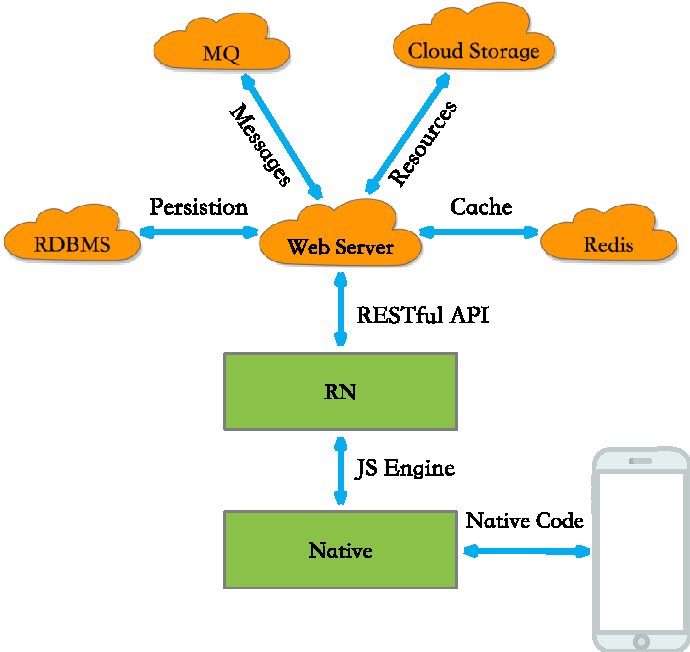
\includegraphics[height=0.6\columnwidth]{components.pdf}
  \caption{系统组件交互图}
  \label{fig:components}
\end{figure}


如\figref{fig_2}所示,系统分别进行服务端、客户端开发(由于使用了前后端分离,前后端可同时开发,互不影响)。服务端架构最上层为中间件层,该层包含AMQ,Redis及Cloud Storage三大中间件。AMQ用于提供消息队列服务,处理邮件、短信等发送业务,Redis负责提供缓存,验证码、Http代理层、客户端所需数据等都缓存于该服务器中。Could Storage提供云存储服务,存储图像、文本等一系列静态资源。SMS服务器、SMTP服务器可用于向用户发送短信、邮件。 

\begin{figure}[htbp]
  \figspace
  \centering
  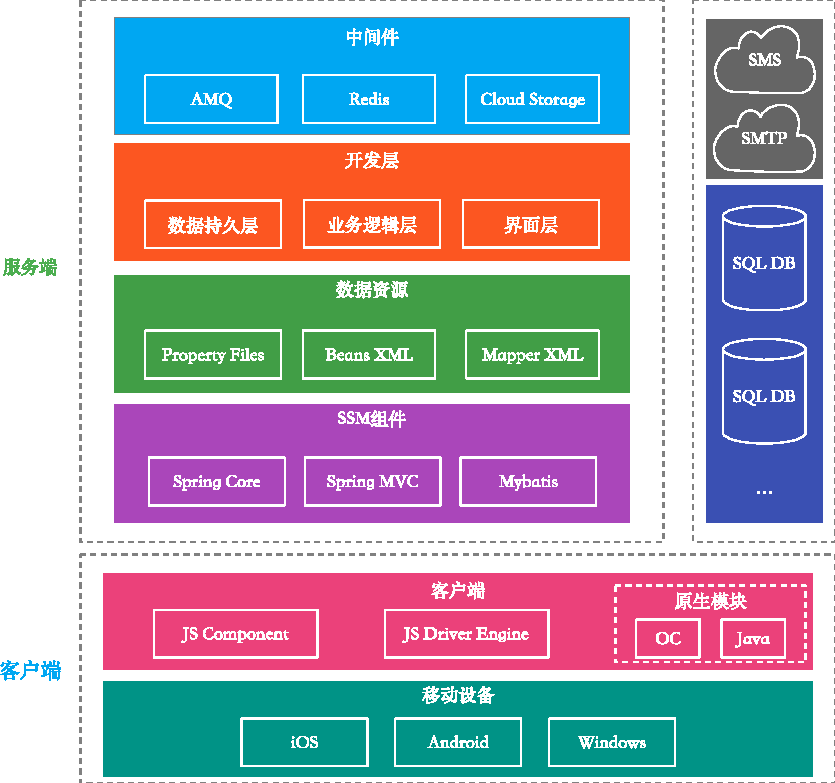
\includegraphics[height=0.8\columnwidth]{framework.pdf}
  \caption{测试融合图}
  \label{fig_2}
\end{figure}

系统下层由开发层提供支撑,开发层与上层中间件通过TCP/IP协议进行数据交换。该层包含数据持久层、业务逻辑层及界面层,数据持久层通过TCP/IP协议向SQL DB服务器获取数据,将数据交由业务逻辑层进一步处理,界面层根据客户端请求,调用业务层处理数据,返回数据。

系统最底层为SSM组件及数据资源层,SSM组件使用文本流调用数据资源层XML等配置信息,提供Web服务。

\begin{enumerate}[(1)]
  \item 这里主要尝试在表格里重置了列表的缩进以后,默认的全局缩进仍然能够生效
  \item 这里主要尝试
  \item 这里主要尝试
  \item 这里主要尝试
  \item 这里主要尝试
\end{enumerate}

客户端架构包含客户端RN层及终端设备层,RN层通过JS Component使用HTTP(S)协议,向服务端获取数据,同时由JS Driver Engine解析数据,并调用原生模块(iOS下为OC模块,Android为Java模块)代码,并使用原生代码及API显示到移动设备中。

\subsection{内部接口设计}

如图 5 3所示,系统实现了不同平台下的解析器。该设计在于扩展不同教务平台,通过使用各自解析器接口,从而实现不同解析策略,最终生成一致数据。
如图 5 3所示,实现了Jxufe及Jxau两个平台解析器,分别适配两个不同平台(部分解析器已省略)。

系统通过JMS Sender向消息队列中写入消息,如图 5 4所示,定义了短信和邮件发送者,分别在系统需要发送短信或邮件时动态调用。

同理,定义JMS Reciever用于处理接收到的消息,根据JMS Sender分别定义了不同的Reciever(如图 5 5所示),用于处理消息队列中不同的消息类别。

\subsection{外部接口设计}
本节根据概要设计,对各模块设计实现,各模块具体实现及流程,由时序图表示,各类依赖,可见类图。

根据概要设计,本节内容对用户管理、用户安全、学生信息、教务信息、失物管理工5大主要模块详细设计

用户管理从注册、登录、信息管理主要三个方面入手。
图 5 6对用户注册作了详细描述,用户输入用户信息,由Web服务器进行处理,当用户未被注册时,对用户所提交密码加密(MD5加盐加密),并存入数据库系统进行存储完成注册,完成注册后,系统对用户自动进行登录状态添加,使用户注册后可直接访问系统,无需再次登录。
 
图 5 7详细描述了用户登录过程,用户在App内输入用户名及密码,由Web服务器验证,服务器从数据库中查询相应用户信息,并获得密文及加密盐值,采用相同算法,再通过比对密码密文,确认是否输入正确用户名及密码。密码验证通过时,系统采用JWT[18],生成用户授权访问令牌,并存储令牌至数据库,同时令牌作为客户端访问唯一授权码。

图 5 8具体展示了系统检验用户登录状态的过程,用户在访问系统需授权访问的服务,都需要使用该流程进行身份认证。客户端在访问授权服务时,必须提供accessToken作为授权访问令牌,系统使用该令牌,结合数据库信息,使用JWT对其进行解密,授权用户进一步访问系统服务。
 
如图 5 9,描述了用户信息修改具体流程,用户通过App对用户个人信息进行编辑,服务器接受用户信息后,通过图 5 8所示验证流程,验证用户登录状态。最后系统更新用户信息至数据库,并删除该用户信息缓存(若存在该缓存,图中已省略该环节)。
 

如图 5 10,当用户首次查看用户信息时,服务器根据App提供参数,向数据库进行数据查询,并缓存用户信息至Redis服务器,除非当用户信息发生更新时,该缓存才失效。当用户再次获取用户信息时,系统直接从Redis缓存中取出该用户信息,而不直接从数据库中读取。该策略采用Redis Cli动态代理技术实现,无需实现具体信息存储代码,使用注解方式,由Spring自行调配动态代理进行信息缓存。
 
如图 5 11所示,用户在进行手机绑定(如图 4 22所示)时,使用手机接收系统所发送的验证码。用户在App中选择获取验证码后,服务器接收到该请求,调用系统业务类,生成验证码并缓存验证码至Redis,同时系统向消息队列中写入发送短信消息,此时Web服务器已经完成响应,App客户端已可以进行其他操作。当系统中消费者已就绪时,立即从消息队列中获取到一条消息,并解析该消息,调用腾讯云SMS短信服务,向目标手机发送短信验证信息。

同理,邮件验证采用几近相同的过程(如图 5 12),向指定邮箱发送验证邮件。不同的是,系统不再调用SMS服务,而转而调用阿里云SMTP服务,向用户邮箱发送验证邮件。
 
如图 5 13所示,当用户收到验证码,并在App客户端输入验证码后,服务器接收用户所输验证码,同时从Redis缓存中获取相应手机或相应邮箱的验证码。系统获得到缓存验证码后,根据其预先设定好的过期时间,判断其是否有效,并与输入值进行比对,若前后验证码相同时,验证即可通过。
 
如图 5 14所示,系统实现了用户在多设备登录时的具体过程,当用户使用App查看已登录设备时,系统首先校验用户访问令牌,以判断该客户端是否为已登录状态。进而系统根据用户信息,获取该用户所有已登录设备,并由App进行展示。

同样的,用户在查看已登录设备时,可尝试对无需登录或未知登录设备进行强行注销操作,如图 5 15所示。

用户选择某台设备(非当前设备)后,可执行删除已登录设备操作,但在此之前,系统首先校验当前App是否为已登录状态,未登录状态不具备删除权限,防止客户端层恶意修改信息。

已登录设备被强制注销后,该设备再次打开App时,将处于未登录状态,其取决于App在运行过程中,会根据如图 5 13所示过程,验证用户状态。
 
当用户登录设备中出现未知设备,则很大可能表示当前账户已存在安全风险,此时用户可进行密码修改,保障账户安全,过程如图 5 16所示。

用户修改密码时需要提供原始密码及新密码,当请求到达服务器后,服务器率先从数据库中获取该用户密码信息,并根据图 5 7所示密码验证过程对原始密码进行认证。原始密码匹配时,采用图 5 6所示密码加密过程,对新密码进行加密,并更新到数据库中。

可知,在密码修改流程中,系统未对Redis中用户信息缓存进行操作,这是因为Redis缓存用户信息并不缓存密码。
 
本节未对找回密码进行详细说明,其基本流程基于图 5 11或图 5 12过程进行安全验证,而后对密码进行重置,完成找回密码。

本节针对用户、学生关系进行实现,根据设计,用户可绑定学生信息,并查看或编辑学生信息。

用户在绑定学生信息时,向系统提供学生信息,并提供教务系统信息,系统使用Http代理业务组件,对学生信息进行认证,认证通过后,用户信息与该学生信息相关联,并访问后续教务信息。过程如图 5 17所示。

当学生更改教务系认证密码后,该系统学生信息必定失效,而无法访问教务信息,此时客户端应提供学生教务用户信息密码修改。在该功能实现中,系统根据学生密码,使用代理认证学生身份,认证成功后更新数据库存储的学生信息(如图 5 18所示)。
 
本节并未对学生信息获取进行详细描述,其基本过程类似于用户信息(如图 5 10)获取,故不再赘述。

本节内容实现了获取教务信息,即课程、考试信息、成绩等功能设计,但上述功能,其基本流程一致,在本节总结概括了所有信息获取流程。
如图 5 20所示,系统根据用户访问令牌,判断用户是否已经登录,并根据令牌获取到用户信息,再根据用户信息获取学生信息,最后使用学生信息,进行平台验证,获取数据后交由解析器(如图 5 3)解析。
 
失物信息管理为本系统扩展功能,本节对该模块包含的失物、评论、回复、关注等角度进行实现。

获取失物流程较为简洁,如图 5 21所示,用户无需鉴权,即可从系统中加载到失物信息。系统对所得失物,按照发布时间进行降序排列。值得注意的是,失物信息加载后,由Redis缓存保存失物信息,直至失物被更新或有新的失物发布,而客户端第二次查询失物时会直接从Redis缓存中读取,无需再次访问数据库。

由于发布失物会对现有失物列表产生改变,因此该操作会清空Redis失物缓存,如图 5 22所示。用户在发布失物时,可选择是否选择图片,当存在图片上传时,首先上传图片至云存储服务器,之后在数据库服务器中存储失物细节及失物图片地址。由于发布失物必须登录用户,因此Web服务器首先验证用户登录状态。

\section{对于代码的引用}

在\lstinline{TEX}中,任何行内的代码,均可使用\lstinline{\lstinline}来进行,其快捷的生命方式为\lstinline!\lstinline!,正如该文本中显示的一样,对于代码文本,其字体发生改变,并以适合代码显示的字体进行显示。

而对于多行字体,其命令也不同,其应当使用\lstinline!listings!中的环境命令进行生命,如下:

\lstset{language=Java}  % 这里先设置语言
\begin{lstlisting}
  var a = Date()
  if (a !=== 0) {
    a = 1
  }
  const b = () => {

  }

  function () {

  }

  b.map(arr, item => {

  })
\end{lstlisting}
若对代码显示风格不满意,可自行进行设定,使用如下命令:

\begin{lstlisting}
  \lstset{language=[LaTeX]TeX,
	texcsstyle=*\bf\color{winered}\ttfamily,
	basicstyle=\xiaosi\ttfamily,
	numbers=none,
	breaklines=true,
	keywordstyle=\bf\color{winered}\ttfamily,
	commentstyle=\color{gray},
	emph={elegantpaper,fontenc,fontspec,xeCJK,FiraMono,xunicode,newtxmath,figure,fig,image,img,table,itemize,enumerate,newtxtext,newtxtt,ctex,microtype,description,times,newtx,booktabs,tabular,PDFLaTeX,XeLaTeX,type1cm,BibTeX},
	emphstyle={\color{frenchplum}},
	morekeywords={DeclareSymbolFont,SetSymbolFont,toprule,midrule,bottomrule,institute,version,includegraphics,setmainfont,setsansfont,setmonofont ,setCJKmainfont,setCJKsansfont,setCJKmonofont,RequirePackage,figref,tabref,email,maketitle,keywords},
	frame=none,
	tabsize=2,
	backgroundcolor=\color{lightgrey}
}
\end{lstlisting}

参见文档:\href{http://texdoc.net/texmf-dist/doc/latex/listings/
listings.pdf}{lstlisting文档}。

\Thanksto

本论在编写过程中,曾受到过来自多方的帮助,感谢论文指导老师胡冬萍老师,在工作之余对论文大纲、定稿等都提出了不少的修改建议,为本文的修改、完善发挥了不可或缺的指导作用。感谢所有为我提供建议及帮助的同学及好友,以及陈积富老师对毕业设计及论文的深切关注,为本论文编写及产品设计提供了技术指导。感谢学院及学校提供的资源及途径,使我可在中国知网等学术库中阅览相关文献,为论文撰写及技术实现提供方向及参考。

此外在本论文的编写过程中,使用了不少开源软件及工具,在此为所有开源组织及个人表示感谢,其对项目构建、实现提供了极大的便捷。



\appendix

\section*{附录第一章}

这是附录内容


\bibliography{ref}
% \bibliographystyle{plain}

\end{document} 
